\documentclass[dissertation.tex]{subfiles}
\begin{document}

\chapter{Model Analysis}

\section{Embeddings}

\subsection{Notes}

\begin{figure}[htpb]
    \centering
    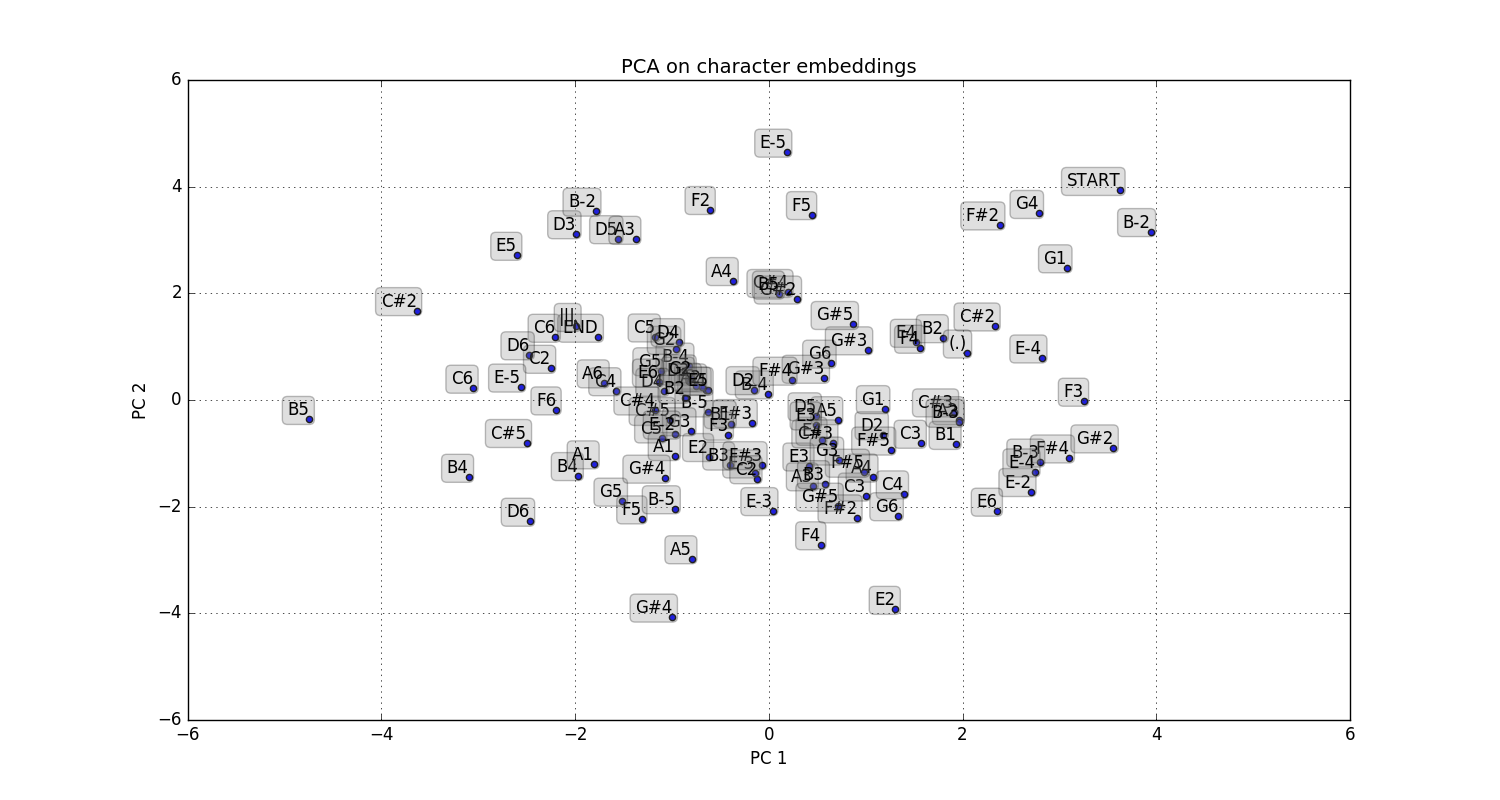
\includegraphics[width=0.8\linewidth]{Figures/PCA-notes.png}
    \caption{PCA embedding of note tokens}
    \label{fig:pca-notes}
\end{figure}

\begin{figure}[htpb]
    \centering
    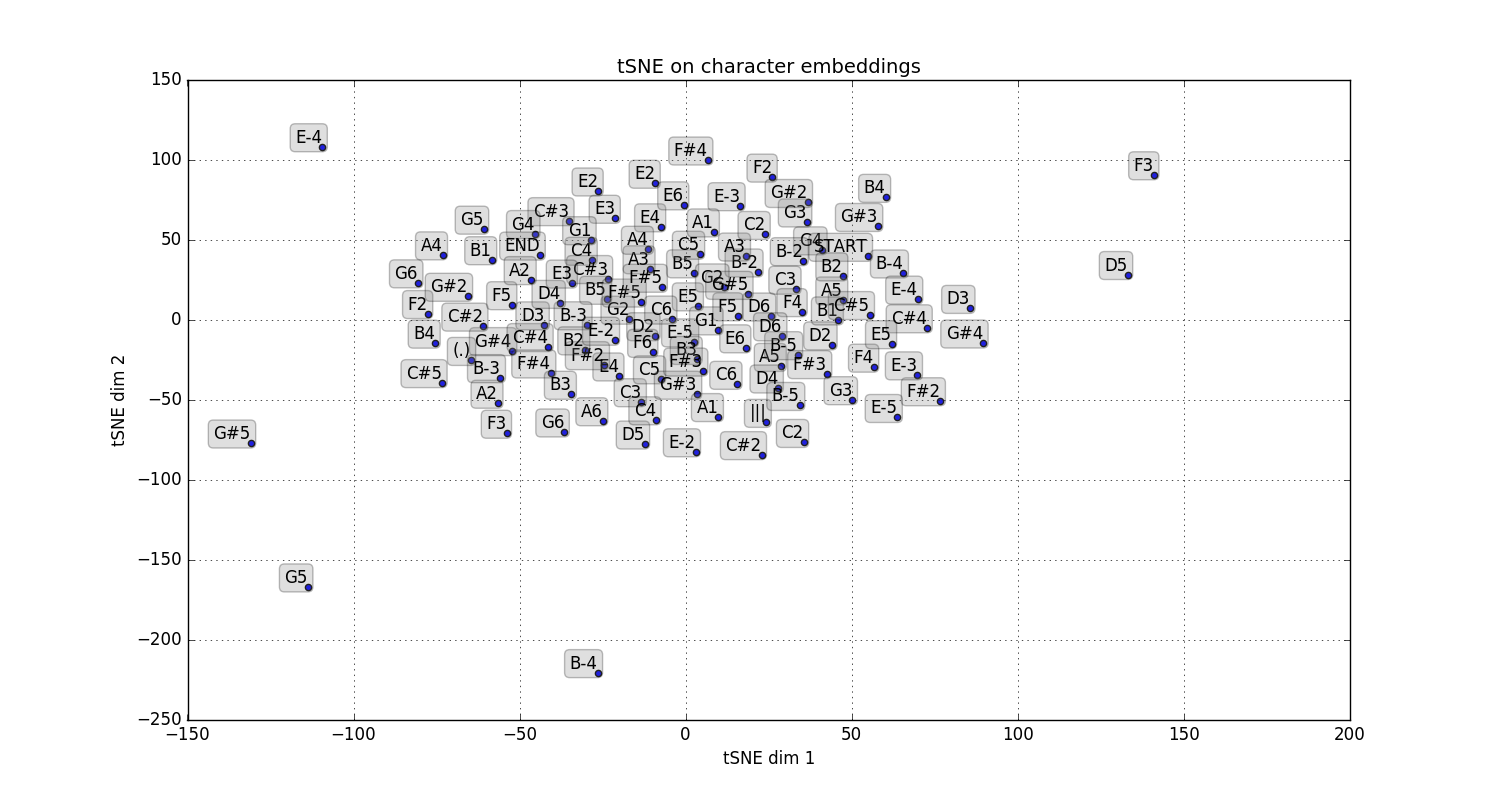
\includegraphics[width=0.8\linewidth]{Figures/tSNE-notes.png}
    \caption{tSNE embedding of note tokens}
    \label{fig:tsne-notes}
\end{figure}

\section{Additional music theory}

\subsection{Meter}

\cite{eck2008learning} first addressed. \emph{Meter} is the sense of a periodic
pattern of strong and weak beats which arise from periodic articulation of
notes in common locations. It is implied in Western music, where bars establish
perodic measures of equal length \cite{handel1993listening}. Meter provides us
with key information about musical structure which can be used to predict chord
changes and repepetition boundaries \cite{cooper1963rhythmic}.

\subsection{Theory tasks}

From \cite{franklin2006recurrent}:

given a dominant 7th chord as input, output in sequence the four chord tones

given each of 14 pairs of five-pitch sequences, output 1 at the end if the second, third, and fourth notes in the sequence are ordered chromatically and otherwise output 0

learn to reproduce one specific 32 note melody of the form AABA, given only the first note as input.

having a pitch-focused network and duration-focused network learn a jazz melody.

\printbibliography

\end{document}
